\documentclass[1p]{elsarticle_modified}
%\bibliographystyle{elsarticle-num}

%\usepackage[colorlinks]{hyperref}
%\usepackage{abbrmath_seonhwa} %\Abb, \Ascr, \Acal ,\Abf, \Afrak
\usepackage{amsfonts}
\usepackage{amssymb}
\usepackage{amsmath}
\usepackage{amsthm}
\usepackage{scalefnt}
\usepackage{amsbsy}
\usepackage{kotex}
\usepackage{caption}
\usepackage{subfig}
\usepackage{color}
\usepackage{graphicx}
\usepackage{xcolor} %% white, black, red, green, blue, cyan, magenta, yellow
\usepackage{float}
\usepackage{setspace}
\usepackage{hyperref}

\usepackage{tikz}
\usetikzlibrary{arrows}

\usepackage{multirow}
\usepackage{array} % fixed length table
\usepackage{hhline}

%%%%%%%%%%%%%%%%%%%%%
\makeatletter
\renewcommand*\env@matrix[1][\arraystretch]{%
	\edef\arraystretch{#1}%
	\hskip -\arraycolsep
	\let\@ifnextchar\new@ifnextchar
	\array{*\c@MaxMatrixCols c}}
\makeatother %https://tex.stackexchange.com/questions/14071/how-can-i-increase-the-line-spacing-in-a-matrix
%%%%%%%%%%%%%%%

\usepackage[normalem]{ulem}

\newcommand{\msout}[1]{\ifmmode\text{\sout{\ensuremath{#1}}}\else\sout{#1}\fi}
%SOURCE: \msout is \stkout macro in https://tex.stackexchange.com/questions/20609/strikeout-in-math-mode

\newcommand{\cancel}[1]{
	\ifmmode
	{\color{red}\msout{#1}}
	\else
	{\color{red}\sout{#1}}
	\fi
}

\newcommand{\add}[1]{
	{\color{blue}\uwave{#1}}
}

\newcommand{\replace}[2]{
	\ifmmode
	{\color{red}\msout{#1}}{\color{blue}\uwave{#2}}
	\else
	{\color{red}\sout{#1}}{\color{blue}\uwave{#2}}
	\fi
}

\newcommand{\Sol}{\mathcal{S}} %segment
\newcommand{\D}{D} %diagram
\newcommand{\A}{\mathcal{A}} %arc


%%%%%%%%%%%%%%%%%%%%%%%%%%%%%5 test

\def\sl{\operatorname{\textup{SL}}(2,\Cbb)}
\def\psl{\operatorname{\textup{PSL}}(2,\Cbb)}
\def\quan{\mkern 1mu \triangleright \mkern 1mu}

\theoremstyle{definition}
\newtheorem{thm}{Theorem}[section]
\newtheorem{prop}[thm]{Proposition}
\newtheorem{lem}[thm]{Lemma}
\newtheorem{ques}[thm]{Question}
\newtheorem{cor}[thm]{Corollary}
\newtheorem{defn}[thm]{Definition}
\newtheorem{exam}[thm]{Example}
\newtheorem{rmk}[thm]{Remark}
\newtheorem{alg}[thm]{Algorithm}

\newcommand{\I}{\sqrt{-1}}
\begin{document}

%\begin{frontmatter}
%
%\title{Boundary parabolic representations of knots up to 8 crossings}
%
%%% Group authors per affiliation:
%\author{Yunhi Cho} 
%\address{Department of Mathematics, University of Seoul, Seoul, Korea}
%\ead{yhcho@uos.ac.kr}
%
%
%\author{Seonhwa Kim} %\fnref{s_kim}}
%\address{Center for Geometry and Physics, Institute for Basic Science, Pohang, 37673, Korea}
%\ead{ryeona17@ibs.re.kr}
%
%\author{Hyuk Kim}
%\address{Department of Mathematical Sciences, Seoul National University, Seoul 08826, Korea}
%\ead{hyukkim@snu.ac.kr}
%
%\author{Seokbeom Yoon}
%\address{Department of Mathematical Sciences, Seoul National University, Seoul, 08826,  Korea}
%\ead{sbyoon15@snu.ac.kr}
%
%\begin{abstract}
%We find all boundary parabolic representation of knots up to 8 crossings.
%
%\end{abstract}
%\begin{keyword}
%    \MSC[2010] 57M25 
%\end{keyword}
%
%\end{frontmatter}

%\linenumbers
%\tableofcontents
%
\newcommand\colored[1]{\textcolor{white}{\rule[-0.35ex]{0.8em}{1.4ex}}\kern-0.8em\color{red} #1}%
%\newcommand\colored[1]{\textcolor{white}{ #1}\kern-2.17ex	\textcolor{white}{ #1}\kern-1.81ex	\textcolor{white}{ #1}\kern-2.15ex\color{red}#1	}

{\Large $\underline{11n_{1}~(K11n_{1})}$}

\setlength{\tabcolsep}{10pt}
\renewcommand{\arraystretch}{1.6}
\vspace{1cm}\begin{tabular}{m{100pt}>{\centering\arraybackslash}m{274pt}}
\multirow{5}{120pt}{
	\centering
	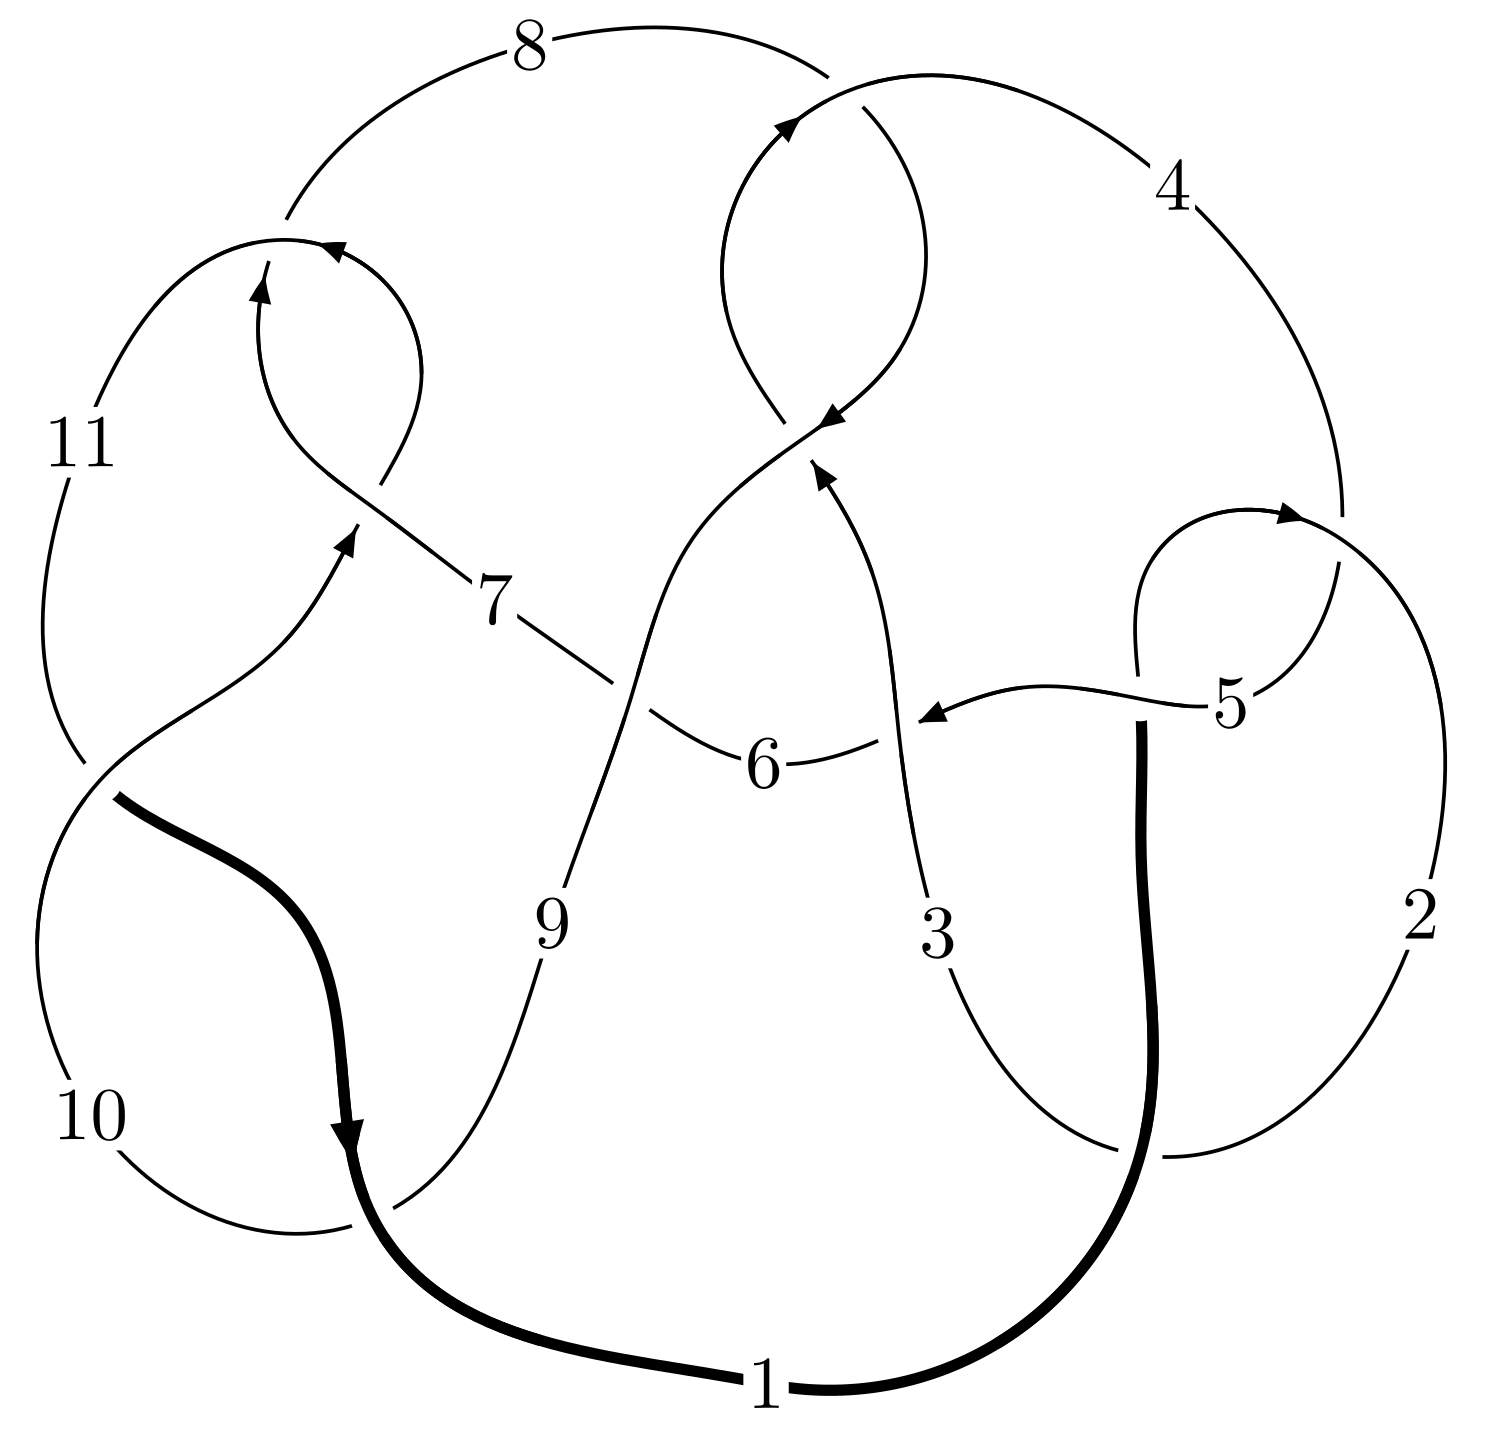
\includegraphics[width=112pt]{../../../GIT/diagram.site/Diagrams/png/617_11n_1.png}\\
\ \ \ A knot diagram\footnotemark}&
\allowdisplaybreaks
\textbf{Linearized knot diagam} \\
\cline{2-2}
 &
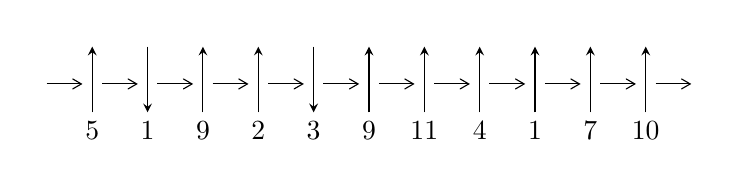
\begin{tikzpicture}[x=20pt, y=17pt]
	% nodes
	\node (C0) at (0, 0) {};
	\node (C1) at (1, 0) {};
	\node (C1U) at (1, +1) {};
	\node (C1D) at (1, -1) {5};

	\node (C2) at (2, 0) {};
	\node (C2U) at (2, +1) {};
	\node (C2D) at (2, -1) {1};

	\node (C3) at (3, 0) {};
	\node (C3U) at (3, +1) {};
	\node (C3D) at (3, -1) {9};

	\node (C4) at (4, 0) {};
	\node (C4U) at (4, +1) {};
	\node (C4D) at (4, -1) {2};

	\node (C5) at (5, 0) {};
	\node (C5U) at (5, +1) {};
	\node (C5D) at (5, -1) {3};

	\node (C6) at (6, 0) {};
	\node (C6U) at (6, +1) {};
	\node (C6D) at (6, -1) {9};

	\node (C7) at (7, 0) {};
	\node (C7U) at (7, +1) {};
	\node (C7D) at (7, -1) {11};

	\node (C8) at (8, 0) {};
	\node (C8U) at (8, +1) {};
	\node (C8D) at (8, -1) {4};

	\node (C9) at (9, 0) {};
	\node (C9U) at (9, +1) {};
	\node (C9D) at (9, -1) {1};

	\node (C10) at (10, 0) {};
	\node (C10U) at (10, +1) {};
	\node (C10D) at (10, -1) {7};

	\node (C11) at (11, 0) {};
	\node (C11U) at (11, +1) {};
	\node (C11D) at (11, -1) {10};
	\node (C12) at (12, 0) {};

	% arrows
	\draw[->,>={angle 60}]
	(C0) edge (C1) (C1) edge (C2) (C2) edge (C3) (C3) edge (C4) (C4) edge (C5) (C5) edge (C6) (C6) edge (C7) (C7) edge (C8) (C8) edge (C9) (C9) edge (C10) (C10) edge (C11) (C11) edge (C12) ;	\draw[->,>=stealth]
	(C1D) edge (C1U) (C2U) edge (C2D) (C3D) edge (C3U) (C4D) edge (C4U) (C5U) edge (C5D) (C6D) edge (C6U) (C7D) edge (C7U) (C8D) edge (C8U) (C9D) edge (C9U) (C10D) edge (C10U) (C11D) edge (C11U) ;
	\end{tikzpicture} \\
\hhline{~~} \\& 
\textbf{Solving Sequence} \\ \cline{2-2} 
 &
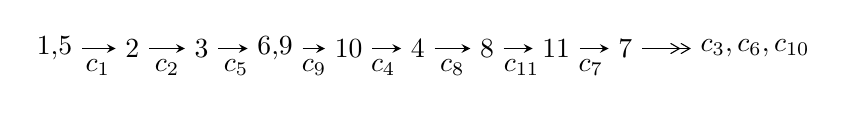
\begin{tikzpicture}[x=25pt, y=7pt]
	% node
	\node (A0) at (-1/8, 0) {1,5};
	\node (A1) at (1, 0) {2};
	\node (A2) at (2, 0) {3};
	\node (A3) at (49/16, 0) {6,9};
	\node (A4) at (33/8, 0) {10};
	\node (A5) at (41/8, 0) {4};
	\node (A6) at (49/8, 0) {8};
	\node (A7) at (57/8, 0) {11};
	\node (A8) at (65/8, 0) {7};
	\node (C1) at (1/2, -1) {$c_{1}$};
	\node (C2) at (3/2, -1) {$c_{2}$};
	\node (C3) at (5/2, -1) {$c_{5}$};
	\node (C4) at (29/8, -1) {$c_{9}$};
	\node (C5) at (37/8, -1) {$c_{4}$};
	\node (C6) at (45/8, -1) {$c_{8}$};
	\node (C7) at (53/8, -1) {$c_{11}$};
	\node (C8) at (61/8, -1) {$c_{7}$};
	\node (A9) at (10, 0) {$c_{3},c_{6},c_{10}$};

	% edge
	\draw[->,>=stealth]	
	(A0) edge (A1) (A1) edge (A2) (A2) edge (A3) (A3) edge (A4) (A4) edge (A5) (A5) edge (A6) (A6) edge (A7) (A7) edge (A8) ;
	\draw[->>,>={angle 60}]	
	(A8) edge (A9);
\end{tikzpicture} \\ 

\end{tabular} \\

\footnotetext{
The image of knot diagram is generated by the software ``\textbf{Draw programme}" developed by Andrew Bartholomew(\url{http://www.layer8.co.uk/maths/draw/index.htm\#Running-draw}), where we modified some parts for our purpose(\url{https://github.com/CATsTAILs/LinksPainter}).
}\phantom \\ \newline 
\centering \textbf{Ideals for irreducible components\footnotemark of $X_{\text{par}}$} 
 
\begin{align*}
I^u_{1}&=\langle 
-2 u^{18}+7 u^{17}+\cdots+4 b+5,\;5 u^{18}-18 u^{17}+\cdots+4 a-5,\;u^{19}-4 u^{18}+\cdots-12 u^2+1\rangle \\
I^u_{2}&=\langle 
- a u+b,\;a^3+a^2 u+a^2+2 a u-1,\;u^2+u+1\rangle \\
\\
\end{align*}
\raggedright * 2 irreducible components of $\dim_{\mathbb{C}}=0$, with total 25 representations.\\
\footnotetext{All coefficients of polynomials are rational numbers. But the coefficients are sometimes approximated in decimal forms when there is not enough margin.}
\newpage
\renewcommand{\arraystretch}{1}
\centering \section*{I. $I^u_{1}= \langle -2 u^{18}+7 u^{17}+\cdots+4 b+5,\;5 u^{18}-18 u^{17}+\cdots+4 a-5,\;u^{19}-4 u^{18}+\cdots-12 u^2+1 \rangle$}
\flushleft \textbf{(i) Arc colorings}\\
\begin{tabular}{m{7pt} m{180pt} m{7pt} m{180pt} }
\flushright $a_{1}=$&$\begin{pmatrix}1\\0\end{pmatrix}$ \\
\flushright $a_{5}=$&$\begin{pmatrix}0\\u\end{pmatrix}$ \\
\flushright $a_{2}=$&$\begin{pmatrix}1\\- u^2\end{pmatrix}$ \\
\flushright $a_{3}=$&$\begin{pmatrix}u^2+1\\- u^2\end{pmatrix}$ \\
\flushright $a_{6}=$&$\begin{pmatrix}- u^5-2 u^3- u\\u^5+u^3+u\end{pmatrix}$ \\
\flushright $a_{9}=$&$\begin{pmatrix}-\frac{5}{4} u^{18}+\frac{9}{2} u^{17}+\cdots+\frac{11}{2} u+\frac{5}{4}\\\frac{1}{2} u^{18}-\frac{7}{4} u^{17}+\cdots-\frac{5}{4} u-\frac{5}{4}\end{pmatrix}$ \\
\flushright $a_{10}=$&$\begin{pmatrix}-0.750000 u^{18}+2.75000 u^{17}+\cdots-19.2500 u^{2}+4.25000 u\\\frac{1}{2} u^{18}-\frac{7}{4} u^{17}+\cdots-\frac{5}{4} u-\frac{5}{4}\end{pmatrix}$ \\
\flushright $a_{4}=$&$\begin{pmatrix}- u\\u^3+u\end{pmatrix}$ \\
\flushright $a_{8}=$&$\begin{pmatrix}-\frac{3}{4} u^{18}+\frac{5}{2} u^{17}+\cdots+\frac{9}{2} u+\frac{3}{4}\\\frac{1}{2} u^{18}-\frac{9}{4} u^{17}+\cdots+\frac{1}{4} u-\frac{3}{4}\end{pmatrix}$ \\
\flushright $a_{11}=$&$\begin{pmatrix}-\frac{1}{4} u^{17}+\frac{3}{4} u^{16}+\cdots+\frac{3}{4} u+\frac{7}{4}\\\frac{1}{4} u^{18}- u^{17}+\cdots- u-\frac{1}{4}\end{pmatrix}$ \\
\flushright $a_{7}=$&$\begin{pmatrix}\frac{1}{4} u^{18}-\frac{3}{4} u^{17}+\cdots-\frac{7}{4} u-1\\-\frac{1}{4} u^{18}+u^{17}+\cdots+2 u+\frac{1}{4}\end{pmatrix}$\\ \flushright $a_{7}=$&$\begin{pmatrix}\frac{1}{4} u^{18}-\frac{3}{4} u^{17}+\cdots-\frac{7}{4} u-1\\-\frac{1}{4} u^{18}+u^{17}+\cdots+2 u+\frac{1}{4}\end{pmatrix}$\\&\end{tabular}
\flushleft \textbf{(ii) Obstruction class $= -1$}\\~\\
\flushleft \textbf{(iii) Cusp Shapes $= 3 u^{18}-\frac{23}{2} u^{17}+43 u^{16}-99 u^{15}+208 u^{14}-350 u^{13}+\frac{1049}{2} u^{12}-708 u^{11}+\frac{1657}{2} u^{10}-926 u^9+884 u^8-803 u^7+\frac{1299}{2} u^6-448 u^5+\frac{615}{2} u^4-136 u^3+\frac{133}{2} u^2-17 u+4$}\\~\\
\newpage\renewcommand{\arraystretch}{1}
\flushleft \textbf{(iv) u-Polynomials at the component}\newline \\
\begin{tabular}{m{50pt}|m{274pt}}
Crossings & \hspace{64pt}u-Polynomials at each crossing \\
\hline $$\begin{aligned}c_{1},c_{4}\end{aligned}$$&$\begin{aligned}
&u^{19}+4 u^{18}+\cdots+12 u^2-1
\end{aligned}$\\
\hline $$\begin{aligned}c_{2}\end{aligned}$$&$\begin{aligned}
&u^{19}+14 u^{18}+\cdots+24 u-1
\end{aligned}$\\
\hline $$\begin{aligned}c_{3},c_{8}\end{aligned}$$&$\begin{aligned}
&u^{19}+u^{18}+\cdots+160 u-64
\end{aligned}$\\
\hline $$\begin{aligned}c_{5}\end{aligned}$$&$\begin{aligned}
&u^{19}-4 u^{18}+\cdots+u-2
\end{aligned}$\\
\hline $$\begin{aligned}c_{6}\end{aligned}$$&$\begin{aligned}
&u^{19}+3 u^{18}+\cdots+2759 u-937
\end{aligned}$\\
\hline $$\begin{aligned}c_{7},c_{10}\end{aligned}$$&$\begin{aligned}
&u^{19}-3 u^{18}+\cdots+u-1
\end{aligned}$\\
\hline $$\begin{aligned}c_{9},c_{11}\end{aligned}$$&$\begin{aligned}
&u^{19}-3 u^{18}+\cdots+11 u-1
\end{aligned}$\\
\hline
\end{tabular}\\~\\
\newpage\renewcommand{\arraystretch}{1}
\flushleft \textbf{(v) Riley Polynomials at the component}\newline \\
\begin{tabular}{m{50pt}|m{274pt}}
Crossings & \hspace{64pt}Riley Polynomials at each crossing \\
\hline $$\begin{aligned}c_{1},c_{4}\end{aligned}$$&$\begin{aligned}
&y^{19}+14 y^{18}+\cdots+24 y-1
\end{aligned}$\\
\hline $$\begin{aligned}c_{2}\end{aligned}$$&$\begin{aligned}
&y^{19}-14 y^{18}+\cdots+612 y-1
\end{aligned}$\\
\hline $$\begin{aligned}c_{3},c_{8}\end{aligned}$$&$\begin{aligned}
&y^{19}+35 y^{18}+\cdots-15360 y-4096
\end{aligned}$\\
\hline $$\begin{aligned}c_{5}\end{aligned}$$&$\begin{aligned}
&y^{19}-42 y^{18}+\cdots+13 y-4
\end{aligned}$\\
\hline $$\begin{aligned}c_{6}\end{aligned}$$&$\begin{aligned}
&y^{19}+89 y^{18}+\cdots+15394803 y-877969
\end{aligned}$\\
\hline $$\begin{aligned}c_{7},c_{10}\end{aligned}$$&$\begin{aligned}
&y^{19}-3 y^{18}+\cdots+11 y-1
\end{aligned}$\\
\hline $$\begin{aligned}c_{9},c_{11}\end{aligned}$$&$\begin{aligned}
&y^{19}+29 y^{18}+\cdots+11 y-1
\end{aligned}$\\
\hline
\end{tabular}\\~\\
\newpage\flushleft \textbf{(vi) Complex Volumes and Cusp Shapes}
$$\begin{array}{c|c|c}  
\text{Solutions to }I^u_{1}& \I (\text{vol} + \sqrt{-1}CS) & \text{Cusp shape}\\
 \hline 
\begin{aligned}
u &= -0.578849 + 0.831148 I \\
a &= -0.236375 - 0.103692 I \\
b &= -0.223009 + 0.136441 I\end{aligned}
 & \phantom{-}0.57171 - 2.29308 I & \phantom{-}0.43534 + 5.97155 I \\ \hline\begin{aligned}
u &= -0.578849 - 0.831148 I \\
a &= -0.236375 + 0.103692 I \\
b &= -0.223009 - 0.136441 I\end{aligned}
 & \phantom{-}0.57171 + 2.29308 I & \phantom{-}0.43534 - 5.97155 I \\ \hline\begin{aligned}
u &= -0.379573 + 1.066790 I \\
a &= -0.384017 + 0.248046 I \\
b &= \phantom{-}0.118852 + 0.503818 I\end{aligned}
 & -1.34954 - 2.72131 I & \phantom{-}3.10172 + 4.42849 I \\ \hline\begin{aligned}
u &= -0.379573 - 1.066790 I \\
a &= -0.384017 - 0.248046 I \\
b &= \phantom{-}0.118852 - 0.503818 I\end{aligned}
 & -1.34954 + 2.72131 I & \phantom{-}3.10172 - 4.42849 I \\ \hline\begin{aligned}
u &= -0.066477 + 0.849480 I \\
a &= \phantom{-}0.390573 - 0.852872 I \\
b &= -0.698534 - 0.388480 I\end{aligned}
 & \phantom{-}0.275217 + 0.309939 I & \phantom{-}6.84413 - 1.19842 I \\ \hline\begin{aligned}
u &= -0.066477 - 0.849480 I \\
a &= \phantom{-}0.390573 + 0.852872 I \\
b &= -0.698534 + 0.388480 I\end{aligned}
 & \phantom{-}0.275217 - 0.309939 I & \phantom{-}6.84413 + 1.19842 I \\ \hline\begin{aligned}
u &= \phantom{-}1.158440 + 0.036055 I \\
a &= -0.02963 - 1.59757 I \\
b &= -0.02328 + 1.85176 I\end{aligned}
 & -13.35980 - 3.50957 I & \phantom{-}4.64823 + 2.14006 I \\ \hline\begin{aligned}
u &= \phantom{-}1.158440 - 0.036055 I \\
a &= -0.02963 + 1.59757 I \\
b &= -0.02328 - 1.85176 I\end{aligned}
 & -13.35980 + 3.50957 I & \phantom{-}4.64823 - 2.14006 I \\ \hline\begin{aligned}
u &= \phantom{-}0.239802 + 1.225750 I \\
a &= \phantom{-}1.218930 - 0.275212 I \\
b &= -0.62964 - 1.42811 I\end{aligned}
 & -5.41009 + 5.31951 I & \phantom{-}2.17850 - 4.32462 I \\ \hline\begin{aligned}
u &= \phantom{-}0.239802 - 1.225750 I \\
a &= \phantom{-}1.218930 + 0.275212 I \\
b &= -0.62964 + 1.42811 I\end{aligned}
 & -5.41009 - 5.31951 I & \phantom{-}2.17850 + 4.32462 I\\
 \hline 
 \end{array}$$\newpage$$\begin{array}{c|c|c}  
\text{Solutions to }I^u_{1}& \I (\text{vol} + \sqrt{-1}CS) & \text{Cusp shape}\\
 \hline 
\begin{aligned}
u &= \phantom{-}0.105421 + 1.309260 I \\
a &= -0.964760 + 0.228937 I \\
b &= \phantom{-}0.401445 + 1.238990 I\end{aligned}
 & -6.74492 - 0.62050 I & \phantom{-}0.784704 + 1.156660 I \\ \hline\begin{aligned}
u &= \phantom{-}0.105421 - 1.309260 I \\
a &= -0.964760 - 0.228937 I \\
b &= \phantom{-}0.401445 - 1.238990 I\end{aligned}
 & -6.74492 + 0.62050 I & \phantom{-}0.784704 - 1.156660 I \\ \hline\begin{aligned}
u &= \phantom{-}0.493476 + 0.148245 I \\
a &= -0.12816 - 2.14991 I \\
b &= -0.255468 + 1.079930 I\end{aligned}
 & -2.12600 - 2.49879 I & \phantom{-}4.77209 + 3.99040 I \\ \hline\begin{aligned}
u &= \phantom{-}0.493476 - 0.148245 I \\
a &= -0.12816 + 2.14991 I \\
b &= -0.255468 - 1.079930 I\end{aligned}
 & -2.12600 + 2.49879 I & \phantom{-}4.77209 - 3.99040 I \\ \hline\begin{aligned}
u &= \phantom{-}0.58478 + 1.39635 I \\
a &= \phantom{-}1.225590 + 0.379250 I \\
b &= -0.18714 - 1.93313 I\end{aligned}
 & -17.6117 + 9.7005 I & \phantom{-}2.62109 - 4.88323 I \\ \hline\begin{aligned}
u &= \phantom{-}0.58478 - 1.39635 I \\
a &= \phantom{-}1.225590 - 0.379250 I \\
b &= -0.18714 + 1.93313 I\end{aligned}
 & -17.6117 - 9.7005 I & \phantom{-}2.62109 + 4.88323 I \\ \hline\begin{aligned}
u &= \phantom{-}0.54417 + 1.43391 I \\
a &= -1.179380 - 0.320996 I \\
b &= \phantom{-}0.18150 + 1.86580 I\end{aligned}
 & -17.9983 + 2.5634 I & \phantom{-}2.10495 - 0.56524 I \\ \hline\begin{aligned}
u &= \phantom{-}0.54417 - 1.43391 I \\
a &= -1.179380 + 0.320996 I \\
b &= \phantom{-}0.18150 - 1.86580 I\end{aligned}
 & -17.9983 - 2.5634 I & \phantom{-}2.10495 + 0.56524 I \\ \hline\begin{aligned}
u &= -0.202383\phantom{ +0.000000I} \\
a &= -1.82553\phantom{ +0.000000I} \\
b &= -0.369456\phantom{ +0.000000I}\end{aligned}
 & \phantom{-}0.846922\phantom{ +0.000000I} & \phantom{-}12.0190\phantom{ +0.000000I}\\
 \hline 
 \end{array}$$\newpage\newpage\renewcommand{\arraystretch}{1}
\centering \section*{II. $I^u_{2}= \langle - a u+b,\;a^3+a^2 u+a^2+2 a u-1,\;u^2+u+1 \rangle$}
\flushleft \textbf{(i) Arc colorings}\\
\begin{tabular}{m{7pt} m{180pt} m{7pt} m{180pt} }
\flushright $a_{1}=$&$\begin{pmatrix}1\\0\end{pmatrix}$ \\
\flushright $a_{5}=$&$\begin{pmatrix}0\\u\end{pmatrix}$ \\
\flushright $a_{2}=$&$\begin{pmatrix}1\\u+1\end{pmatrix}$ \\
\flushright $a_{3}=$&$\begin{pmatrix}- u\\u+1\end{pmatrix}$ \\
\flushright $a_{6}=$&$\begin{pmatrix}-1\\0\end{pmatrix}$ \\
\flushright $a_{9}=$&$\begin{pmatrix}a\\a u\end{pmatrix}$ \\
\flushright $a_{10}=$&$\begin{pmatrix}a u+a\\a u\end{pmatrix}$ \\
\flushright $a_{4}=$&$\begin{pmatrix}- u\\u+1\end{pmatrix}$ \\
\flushright $a_{8}=$&$\begin{pmatrix}a\\a u\end{pmatrix}$ \\
\flushright $a_{11}=$&$\begin{pmatrix}- a^2+1\\- a^2 u- a^2\end{pmatrix}$ \\
\flushright $a_{7}=$&$\begin{pmatrix}a^2 u-1\\- a^2 u- a^2\end{pmatrix}$\\ \flushright $a_{7}=$&$\begin{pmatrix}a^2 u-1\\- a^2 u- a^2\end{pmatrix}$\\&\end{tabular}
\flushleft \textbf{(ii) Obstruction class $= 1$}\\~\\
\flushleft \textbf{(iii) Cusp Shapes $= -5 a^2 u-6 a^2-5 a u- a+u+14$}\\~\\
\newpage\renewcommand{\arraystretch}{1}
\flushleft \textbf{(iv) u-Polynomials at the component}\newline \\
\begin{tabular}{m{50pt}|m{274pt}}
Crossings & \hspace{64pt}u-Polynomials at each crossing \\
\hline $$\begin{aligned}c_{1},c_{2},c_{5}\end{aligned}$$&$\begin{aligned}
&(u^2+u+1)^3
\end{aligned}$\\
\hline $$\begin{aligned}c_{3},c_{8}\end{aligned}$$&$\begin{aligned}
&u^6
\end{aligned}$\\
\hline $$\begin{aligned}c_{4}\end{aligned}$$&$\begin{aligned}
&(u^2- u+1)^3
\end{aligned}$\\
\hline $$\begin{aligned}c_{6},c_{9}\end{aligned}$$&$\begin{aligned}
&(u^3+u^2+2 u+1)^2
\end{aligned}$\\
\hline $$\begin{aligned}c_{7}\end{aligned}$$&$\begin{aligned}
&(u^3- u^2+1)^2
\end{aligned}$\\
\hline $$\begin{aligned}c_{10}\end{aligned}$$&$\begin{aligned}
&(u^3+u^2-1)^2
\end{aligned}$\\
\hline $$\begin{aligned}c_{11}\end{aligned}$$&$\begin{aligned}
&(u^3- u^2+2 u-1)^2
\end{aligned}$\\
\hline
\end{tabular}\\~\\
\newpage\renewcommand{\arraystretch}{1}
\flushleft \textbf{(v) Riley Polynomials at the component}\newline \\
\begin{tabular}{m{50pt}|m{274pt}}
Crossings & \hspace{64pt}Riley Polynomials at each crossing \\
\hline $$\begin{aligned}c_{1},c_{2},c_{4}\\c_{5}\end{aligned}$$&$\begin{aligned}
&(y^2+y+1)^3
\end{aligned}$\\
\hline $$\begin{aligned}c_{3},c_{8}\end{aligned}$$&$\begin{aligned}
&y^6
\end{aligned}$\\
\hline $$\begin{aligned}c_{6},c_{9},c_{11}\end{aligned}$$&$\begin{aligned}
&(y^3+3 y^2+2 y-1)^2
\end{aligned}$\\
\hline $$\begin{aligned}c_{7},c_{10}\end{aligned}$$&$\begin{aligned}
&(y^3- y^2+2 y-1)^2
\end{aligned}$\\
\hline
\end{tabular}\\~\\
\newpage\flushleft \textbf{(vi) Complex Volumes and Cusp Shapes}
$$\begin{array}{c|c|c}  
\text{Solutions to }I^u_{2}& \I (\text{vol} + \sqrt{-1}CS) & \text{Cusp shape}\\
 \hline 
\begin{aligned}
u &= -0.500000 + 0.866025 I \\
a &= -1.239560 + 0.467306 I \\
b &= \phantom{-}0.215080 - 1.307140 I\end{aligned}
 & -3.02413 + 0.79824 I & \phantom{-}2.74410 - 0.29766 I \\ \hline\begin{aligned}
u &= -0.500000 + 0.866025 I \\
a &= \phantom{-}1.024480 - 0.839835 I \\
b &= \phantom{-}0.215080 + 1.307140 I\end{aligned}
 & -3.02413 - 4.85801 I & \phantom{-}4.03424 + 5.28153 I \\ \hline\begin{aligned}
u &= -0.500000 + 0.866025 I \\
a &= -0.284920 - 0.493496 I \\
b &= \phantom{-}0.569840\phantom{ +0.000000I}\end{aligned}
 & \phantom{-}1.11345 - 2.02988 I & \phantom{-}12.72167 + 1.07831 I \\ \hline\begin{aligned}
u &= -0.500000 - 0.866025 I \\
a &= \phantom{-}1.024480 + 0.839835 I \\
b &= \phantom{-}0.215080 - 1.307140 I\end{aligned}
 & -3.02413 - 0.79824 I & \phantom{-}2.74410 + 0.29766 I \\ \hline\begin{aligned}
u &= -0.500000 - 0.866025 I \\
a &= -1.239560 - 0.467306 I \\
b &= \phantom{-}0.215080 + 1.307140 I\end{aligned}
 & -3.02413 + 4.85801 I & \phantom{-}4.03424 - 5.28153 I \\ \hline\begin{aligned}
u &= -0.500000 - 0.866025 I \\
a &= -0.284920 + 0.493496 I \\
b &= \phantom{-}0.569840\phantom{ +0.000000I}\end{aligned}
 & \phantom{-}1.11345 + 2.02988 I & \phantom{-}12.72167 - 1.07831 I\\
 \hline 
 \end{array}$$\newpage
\newpage\renewcommand{\arraystretch}{1}
\centering \section*{ III. u-Polynomials}
\begin{tabular}{m{50pt}|m{274pt}}
Crossings & \hspace{64pt}u-Polynomials at each crossing \\
\hline $$\begin{aligned}c_{1}\end{aligned}$$&$\begin{aligned}
&((u^2+u+1)^3)(u^{19}+4 u^{18}+\cdots+12 u^2-1)
\end{aligned}$\\
\hline $$\begin{aligned}c_{2}\end{aligned}$$&$\begin{aligned}
&((u^2+u+1)^3)(u^{19}+14 u^{18}+\cdots+24 u-1)
\end{aligned}$\\
\hline $$\begin{aligned}c_{3},c_{8}\end{aligned}$$&$\begin{aligned}
&u^6(u^{19}+u^{18}+\cdots+160 u-64)
\end{aligned}$\\
\hline $$\begin{aligned}c_{4}\end{aligned}$$&$\begin{aligned}
&((u^2- u+1)^3)(u^{19}+4 u^{18}+\cdots+12 u^2-1)
\end{aligned}$\\
\hline $$\begin{aligned}c_{5}\end{aligned}$$&$\begin{aligned}
&((u^2+u+1)^3)(u^{19}-4 u^{18}+\cdots+u-2)
\end{aligned}$\\
\hline $$\begin{aligned}c_{6}\end{aligned}$$&$\begin{aligned}
&((u^3+u^2+2 u+1)^2)(u^{19}+3 u^{18}+\cdots+2759 u-937)
\end{aligned}$\\
\hline $$\begin{aligned}c_{7}\end{aligned}$$&$\begin{aligned}
&((u^3- u^2+1)^2)(u^{19}-3 u^{18}+\cdots+u-1)
\end{aligned}$\\
\hline $$\begin{aligned}c_{9}\end{aligned}$$&$\begin{aligned}
&((u^3+u^2+2 u+1)^2)(u^{19}-3 u^{18}+\cdots+11 u-1)
\end{aligned}$\\
\hline $$\begin{aligned}c_{10}\end{aligned}$$&$\begin{aligned}
&((u^3+u^2-1)^2)(u^{19}-3 u^{18}+\cdots+u-1)
\end{aligned}$\\
\hline $$\begin{aligned}c_{11}\end{aligned}$$&$\begin{aligned}
&((u^3- u^2+2 u-1)^2)(u^{19}-3 u^{18}+\cdots+11 u-1)
\end{aligned}$\\
\hline
\end{tabular}\newpage\renewcommand{\arraystretch}{1}
\centering \section*{ IV. Riley Polynomials}
\begin{tabular}{m{50pt}|m{274pt}}
Crossings & \hspace{64pt}Riley Polynomials at each crossing \\
\hline $$\begin{aligned}c_{1},c_{4}\end{aligned}$$&$\begin{aligned}
&((y^2+y+1)^3)(y^{19}+14 y^{18}+\cdots+24 y-1)
\end{aligned}$\\
\hline $$\begin{aligned}c_{2}\end{aligned}$$&$\begin{aligned}
&((y^2+y+1)^3)(y^{19}-14 y^{18}+\cdots+612 y-1)
\end{aligned}$\\
\hline $$\begin{aligned}c_{3},c_{8}\end{aligned}$$&$\begin{aligned}
&y^6(y^{19}+35 y^{18}+\cdots-15360 y-4096)
\end{aligned}$\\
\hline $$\begin{aligned}c_{5}\end{aligned}$$&$\begin{aligned}
&((y^2+y+1)^3)(y^{19}-42 y^{18}+\cdots+13 y-4)
\end{aligned}$\\
\hline $$\begin{aligned}c_{6}\end{aligned}$$&$\begin{aligned}
&((y^3+3 y^2+2 y-1)^2)(y^{19}+89 y^{18}+\cdots+1.53948\times10^{7} y-877969)
\end{aligned}$\\
\hline $$\begin{aligned}c_{7},c_{10}\end{aligned}$$&$\begin{aligned}
&((y^3- y^2+2 y-1)^2)(y^{19}-3 y^{18}+\cdots+11 y-1)
\end{aligned}$\\
\hline $$\begin{aligned}c_{9},c_{11}\end{aligned}$$&$\begin{aligned}
&((y^3+3 y^2+2 y-1)^2)(y^{19}+29 y^{18}+\cdots+11 y-1)
\end{aligned}$\\
\hline
\end{tabular}
\vskip 2pc
\end{document}